
\section{Theory}\label{sec:theory}

This section introduces the mathematical theory behind the recommendation model, a summary of the supervised learning process and some theory about the evaluation metrics \textit{Precision}, \textit{Recall} and \textit{F-measure}. Then a brief overview of optimization techniques is given and then explanation of the recommendation algorithms \textit{link-analysis} and \textit{katz-eig}. The section is finished by a brief mention of unsupervised learning techniques, mainly about clustering.

%This section introduces the mathematical theory behind the recommendation model, the evaluation of recommendations and a summary of the supervised learning process.
%\Warning[TODO]{ Make sure these are up to date }

This is the basic process of producing recommendations:

\begin{enumerate}
    \item Given an interaction history $h_{u, i}$ and algorithm specific parameters the recommendation algorithm produce recommendations $p_{u, i}$.
    \item The recommendations $p_{u, i}$, which are real values, are converted to binary recommendations $r_{u, i}$.
\end{enumerate}

The process of parameter tuning used is as follows:

\begin{enumerate}
    \item Split the interaction matrix $A$ into a training set $A_{train}$, a validation set $A_{val}$ and a test set $A_{test}$.
    \item Evaluate different parameters by producing recommendations with $A_{train}$ and evaluating them against $A_{val}$ or $A_{test}$ with respect to \textit{F-measure}.
    \item Select the best performing parameters with respect to \textit{F-measure}.
\end{enumerate}


\subsection{Model}\label{sec:background:theory:model}

Given a set of users $U$, a set of items $I$ and an interaction history $h_{u, i}$ given in \textit{unweighted binary form}

\begin{equation}\label{eq:hist}
    h_{u, i} = \begin{cases}
        1 \quad \text{if user $u$ has interacted with item $i$} \\
        0 \quad \text{otherwise}
    \end{cases}
\end{equation}

the \textit{recommender problem} is defined by producing a set of recommendations $r_{u, i}$

\begin{equation}\label{eq:binrec}
    r_{u, i} = \begin{cases}
        1 \quad \text{if item $i$ is recommended to user $u$} \\
        0 \quad \text{otherwise}
    \end{cases}
\end{equation}

to maximize the probability that user $u$ will want to interact with item $i$ in the future, for all users and items.  When $r_{u, i}$ is binary this is a \textit{binary classification} problem. This definition is applicable for \textit{implicit feedback} systems which passively track different sorts of user behaviour. For example link following, interaction time and purchase history.

The recommender problem can be extended to the \textit{Top-N recommender problem} by introducing constraints \eqref{eq:constrain_N} which states that only $N$ recommendations can be presented for each user.

\begin{equation}\label{eq:constrain_N}
    \sum_i r_{u, i} \leq N \quad \forall u
\end{equation}


A variation of the recommender problem is when the interaction history is in \textit{weighted form}, when the values increase with each interaction

\begin{equation}\label{eq:whist}
    h_{u, i} = \begin{cases}
        x \quad \text{user $u$ has interacted $x$ times with item $i$} \\
        0 \quad \text{otherwise}
    \end{cases}
\end{equation}

for example $h_{u, i} = 2$ means that the user $u$ has interacted with item $i$ 2 times. It is possible to allow \textit{implicit feedback} systems to log partial interactions, so $h_{u, i} = 0.7$ could mean that user $u$ has watched 70\% of the movie $i$, in the context of movie watching. \citep{hu2008collaborative}

The converse of \textit{implicit feedback} is \textit{explicit feedback} where the users give direct input regarding their preferences, for example with movie ratings or with likes and dislikes.  Here the definition of the interaction history $h_{u, i}$ is the users' rating history.

\begin{equation}
    h_{u, i} = \begin{cases}
        x \quad \text{the rating $x$ user $u$ gave item $i$} \\
        \emptyset \quad \text{if the user $u$ did not rate item $i$}
    \end{cases}
\end{equation}

\Warning[TODO]{ Uses h for all equations? }

With ratings $r_{u, i}$ changes to $r_{u, i} = \hat{x}$ where $\hat{x}$ is the rating user $u$ is predicted to give item $i$.


\subsection{Prediction}\label{sec:background:theory:pred}

The algorithms which produce binary classification recommendations produce predictions for each user-item pair, denoted $p_{u, i}$. Generally the higher the value of $p_{u, i}$ the more likely is it that user $u$ will interact with item $i$. In a classification context when the interaction history describes ratings the value corresponds to the predicted ratings user $u$ would give $i$. For example if $p_{u, i} = 3.8$ means a user $u$ is predicted to rate item $i$ a 4, given discrete ratings between 1 and 5.

Some algorithms also output a confidence value $c_{u, i}$ which denotes how certain the predicted values are. This is relevant when predicting ratings, for example $p_{u, i} = 4.0$ may seem like a surely predicted 4 rating but a low value of $c_{u, i}$ means we might not want to recommend that item anyway.



\subsection{Supervised learning}\label{sec:background:theory:suplearn}

The task of \textit{supervised learning} is given a \textit{training set} with input-output pairs discover a function, the hypothesis, which approximates the input-output mapping.  To measure the accuracy of the hypothesis match it against a \textit{test set} with input-output pairs distinct from the training set.
\citep{norvigAI}

There can be multiple available models for the hypothesis, for example if the hypothesis is a polynomial function of the form 

\begin{equation}
f(x) = a_n x^n + a_{n - 1} x^{n - 1} + ... + a_2 x^2 + a_1 x + a_0
\end{equation}

then the polynomial degree $n = 1, 2, 3, ...$ represents different possible models for the hypothesis \citep{norvigAI}. Other examples include the number of layers and the number of units in a neural network or the rank of a low rank approximation.
\Warning[TODO]{ examples need ref }

The different models represents the complexity of the hypothesis. A more complex model can make a better fit to the training data but that introduces the problem of \textit{overfitting} where the hypothesis fits the training data \textit{too} well and it will not fit the test data.
\citep{norvigAI}

\textit{Model selection} is thus performed by evaluating performance on a \textit{validation set} (sometimes called a \textit{cross-validation set}). The reason not to both choose the model and evaluate the accuracy using the test set is that then we will have overfit the test set as we both choose the best model and then calculate the accuracy \textit{on the already best fit}.
\citep{norvigAI}

In practice you have a set of data which you randomly split into the training, test and validation sets. The recommended ratio differs, common recommendations include 60/20/20, 80/10/10, or 70/15/15 \footnote{As recommended by Andrew Ng, Stanford. \url{https://class.coursera.org/ml-006}} depending on domain and the size of the available data set. The training set is larger than the others.

If there is no need for a validation set, which can be the case if there are no models to choose from, common training/test set ratios include 70/30, 80/20 \cite{hu2008collaborative} or 90/10.
\Warning[TODO]{ More ref! }


In summary machine learning for supervised learning is done in a couple of steps:

\begin{description}
    \item[Preface] Split data set into training, test and validation sets.
    \item[Training phase] Train the hypothesis using the training set.
    \item[Model selection] Select model using the validation set. (Optional)
    \item[Evaluation] Estimate the accuracy using the test set.
    \item[Application] Apply the developed model to real world data and get results.
\end{description}

Another way to combat overfitting is with \textit{regularization}. Regularization searches for a hypothesis directly penalizes complexity.  Regularization still needs to select $\lambda$ using model selection.
\citep{norvigAI}


\section{Evaluation}\label{sec:method:eval}

Recommendation quality was evaluated using \textit{Precision}, \textit{Recall} and \textit{F-measure} with top-10 recommendations. Focus was on \textit{F-measure} as a combined measure of \textit{Precision} and \textit{Recall}.

The following steps describes the steps taken to produce evaluations given the training, validation and test sets $A_{train}$, $A_{val}$ and $A_{test}$:

\begin{enumerate}
    \item Produce recommendation predictions $p_{u, i}$ from $A_{train}$ with the chosen algorithm.
    \item Transform $p_{u, i}$ to a set of binary recommendations $r_{u, i}$ using the top-10 most predicted items for each user, by the process described in \chapterref{cha:theory}.
    \item Evaluate \textit{F-measure}, as described in \sectionref{sec:background:theory:eval}, with $e_{u, i}$ representing $A_{val}$ or $A_{test}$, depending on which set to evaluate against.
\end{enumerate}

If not explicitly noted, the evaluation set was the test set.



\section{Optimization}\label{sec:background:opt}

Most supervised learning algorithms try to minimize a cost function during the learning phase. This function computes a value given some learned parameters and it can vary with different algorithms. The cost function does not make a comparison between two different sets but computes a metric from a single set.

A simple cost function (without regularization) could be defined as

\begin{equation}
    \min_{r_{u, i}} \sum_{h_{u,i} \text{ is known} } (h_{u, i} - r_{u, i})^2
\end{equation}

A typical recommendation model associates each user $u$ with a user-factors vector $x_u$ and each item $i$ with an item-factors vector $y_i$ such that $r_{u, i} = x_u^T y_i$
\citep{hu2008collaborative}. In such a case a cost function could be defined as

\begin{equation}
    \min_{x_*, y_*} \sum_{h_{u,i} \text{ is known} } (h_{u, i} - x_{u}^T y_i)^2
\end{equation}

where the the optimization objective is $x_u$ and $y_i$. Usually stochastic gradient descent is used to find the parameters \cite{hu2008collaborative}. With regularization a possible cost function could be

\begin{equation}\label{eq:exreg}
    \min_{x_*, y_*} \sum_{h_{u,i} \text{ is known} } (h_{u, i} - x_{u}^T y_i)^2 + \lambda(\|x_u\|^2 + \|y_i\|^2)
\end{equation}

where $\lambda$ is the regularization hyperparameter found using \textit{model selection}. This directly penalizes larger values of $x_u$ and $y_i$ which in this case corresponds to an increase in complexity.

Metrics such as \textit{F-measure} can be used directly as optimization criteria if a suitable cost function is hard to find. It is also a common way of evaluating different models during model selection, the hyperparameter $\lambda$ in equation \eqref{eq:exreg} can be evaluated in this way
\footnote{Machine Learning, Stanford. \url{https://class.coursera.org/ml-006}}
.

There are a couple of generic optimization techniques used for optimizing cost functions and selecting parameters via recommender quality metrics such as \textit{F-measure}. In all cases the problem consists of minimizing or maximizing a target function. What follows are short descriptions of some common techniques:


\subsubsection{Grid search}

Grid search is a straightforward search technique which evaluates the function over a limited parameter space. This is a recommended approach for selecting the regularization parameter $\lambda$
\footnote{Suggested by Andrew Ng in his lectures on Machine Learning. \url{https://class.coursera.org/ml-006}}.

Grid search is easily parallelized but it suffers from the curse of dimensionality, where it's particularly slow if used to optimize multiple parameters.


\subsubsection{Random search}

Grid search is exhaustive and possibly expensive, random search with a fixed limit of samples has been shown to be more effective in high-dimension spaces \citep{bergstra2012random}. Random search is easily parallelized but lacks guidance.


\subsubsection{Hill climbing}

Is a technique for finding a local optima from a given starting point. The neighbours of the current state is examined and the state is moved to the neighbour with a better function value until a local optima has been found. Variations for continuous functions exists which decrease the step size dynamically to increase the precision. \citep{norvigAI}


\subsubsection{Gradient based approaches}

Variations of gradient based optimization techniques such as stochastic gradient descent can be used to optimize functions given that a gradient can be found. The search is similar to that of hill climbing, but is guided by the gradient and optimizes for a local optima.  This is a fast and popular method for optimizing learning parameters.
\cite{hu2008collaborative}


\subsubsection{Simulated annealing}

Simulated annealing is a probabilistic heuristic optimization technique used for finding global optima in a limited search space. It works by randomly jumping to neighbouring points with decreasing probability until it converges on a local optima. However it is more likely to find a better local optima than a gradient based approach. \citep{norvigAI}


\subsubsection{Bayesian optimization}

Bayesian optimization develops a statistical model over the function space and evaluates the function sparsely which balances exploration and exploitation.  With \textit{Gaussian process priors}, a form of statistical modeling of a function, Bayesian optimization has been shown to give better results with fewer evaluations than grid search. \citep{snoek2012practical}



\section{The link-analysis algorithm}\label{sec:linkanalysis}

%\textit{Cleanup, mostly description from article. Reduce information?}

The \textit{link-analysis} algorithm, as presented by \cite{huang2004link} and further discussed in \cite{huang2007comparison}. See the articles for more information and in-depth examples. What follows is a condensed description of how the algorithm works.

The algorithm is an adaptation of HITS \cite{kleinberg1999authoritative} which is a web page ranking algorithm to the recommendation domain. The original algorithm distinguish between \textit{Authoritative} pages which definitely contain high-quality information and \textit{Hub} pages which are comprehensive lists of links to authoritative pages. \citep{huang2007comparison}

The adaptation to the recommendation domain is achieved by introducing the \textit{product representativeness} score $\PR$ and the \textit{consumer representativeness} score $\CR$.

The \textit{product representativeness} score $\PR(i, u)$ can be seen as a measure of the item $i$'s level of interest with respect to user $u$, or in other words $i$'s authority of $u$'s interests in $i$.

The \textit{consumer representativeness} score $\CR(u, \hat{u})$ measures how well $u$ as a hub for $\hat{u}$ associates with products of interests to $\hat{u}$.

If $h_{u, i}$ is the user-item interaction history as defined by \ref{eq:hist} and $h$ is the interaction matrix then a recursive definition of the authority and hub scores can be defined as

\begin{equation}
    \PR = h' * \CR
\end{equation}

\begin{equation}
    \CR = B * \PR + \CR_0
\end{equation}

Where $B$ is a matrix such that:

\begin{equation}
    B_{u, i} = \frac{ h_{u, i} }{ \left(\sum_{i} h_{u, i}\right)^\gamma }
\end{equation}

Meaning $B$ normalizes the representativeness score a costumer receives from linked products by dividing it with the total number of products the customer is linked to.  $\gamma$ controls the extent to which a consumer is penalized for making many purchases.

$\CR_0$ is defined as

\begin{equation}
    \CR_{i, j}^0 = \begin{cases}
        \eta \quad \text{if } \; i = j \\
        0    \quad \text{otherwise}
    \end{cases}
\end{equation}

in other words $\CR_0 = \eta * I_M$ where $I_M$ is an $M x M$ identity matrix and $M$ is the number of users.  It is included to maintain the high representativeness score for the target users themselves. This also necessitates a normalization step to keep the values on a consistent level.

In summary the \textit{link-analysis} algorithm follow these steps:

\begin{enumerate}
    \item Construct the interaction matrix $A$ and the associating matrix $B$.

    \item Set $\CR_0 = \eta * I_M$.
    \item At each iteration $t = 1, \ldots, t_{max}$ perform:

        \begin{enumerate}
            \item $\PR_t = h' * \CR_{t- 1}$
            \item $\CR_t = B * \PR_t$
            \item Normalize $\CR_t$ so each column adds up to 1
            \item $\CR_t = \CR_t + \CR_0$
        \end{enumerate}

        Repeat until convergence.

    \item Predicted user-item interaction is given by $\mathit{pval} = \PR'$.

\end{enumerate}

There are two parameters to the algorithm: $\gamma$ and $\eta$.
%\Warning[TODO]{ Describe them, what's their purpose }



\subsection{katz-eig}

There are two parameters to \textit{katz-eig}: $\beta$, the link diminishing factor and $K$ specifying the $K$-rank approximation. $\beta$ is a continous value satisfying $0 < \beta \leq \frac{1}{\|A_{train}\|_2}$. If $\beta = 0$ then the algorithm will only output 0 and if $\beta > \frac{1}{\|A_{train}\|_2}$ the iterations will not converge. $K > 0$ is a discrete value.

What follows is plots over both of the parameters $K$ and $\beta$. The plots are evaluated using \textit{F-measure} w.r.t. the test set using top-10 recommendations.

\begin{figure}[h!]
\centering
\begin{minipage}{.5\textwidth}
    \centering
    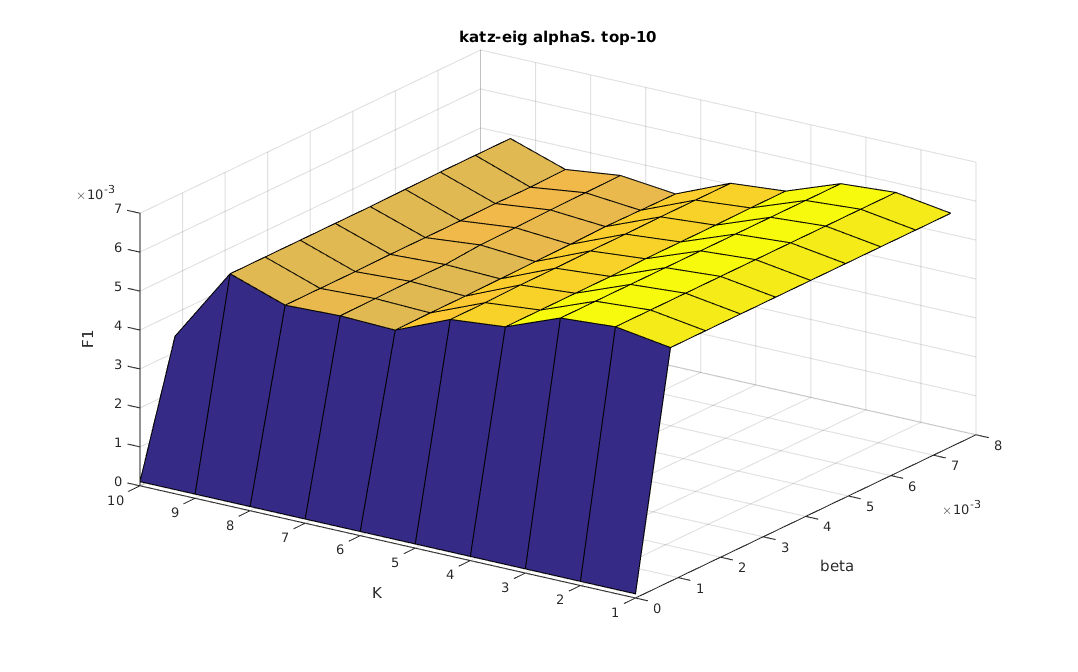
\includegraphics[width=\linewidth]{fig/katzeig_beta_k/alphaS_katzeig.png}
    \captionof{figure}{\textit{alphaS}}
\end{minipage}%
\begin{minipage}{.5\textwidth}
    \centering
    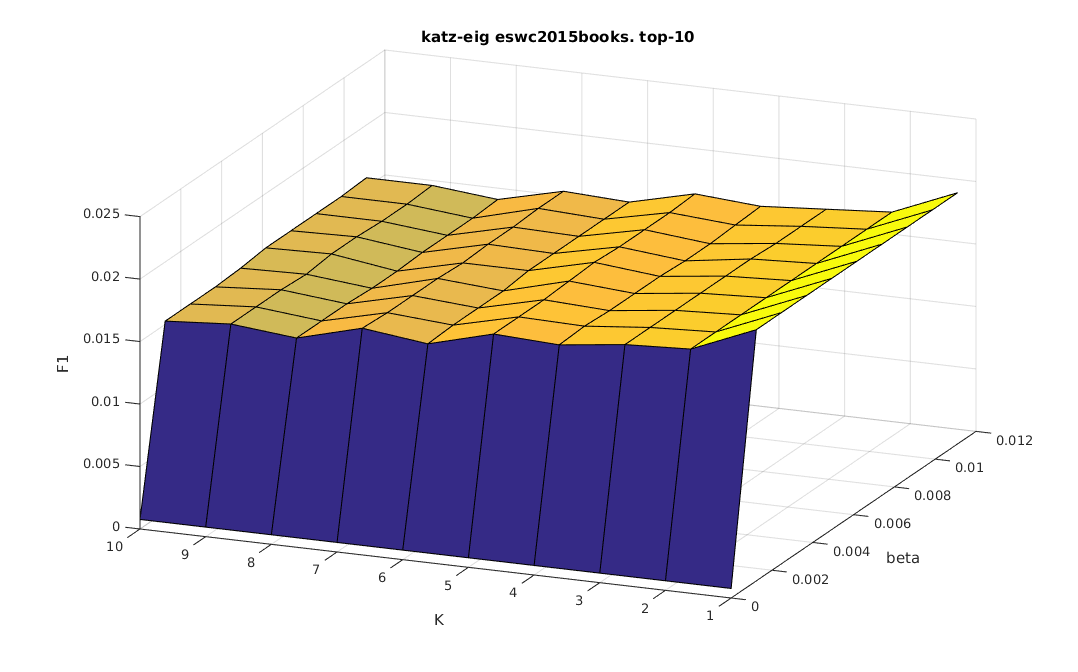
\includegraphics[width=\linewidth]{fig/katzeig_beta_k/eswc2015books_katzeig.png}
    \captionof{figure}{\textit{eswc2015books}}
\end{minipage}
\end{figure}

\begin{figure}[h!]
\centering
\begin{minipage}{.5\textwidth}
    \centering
    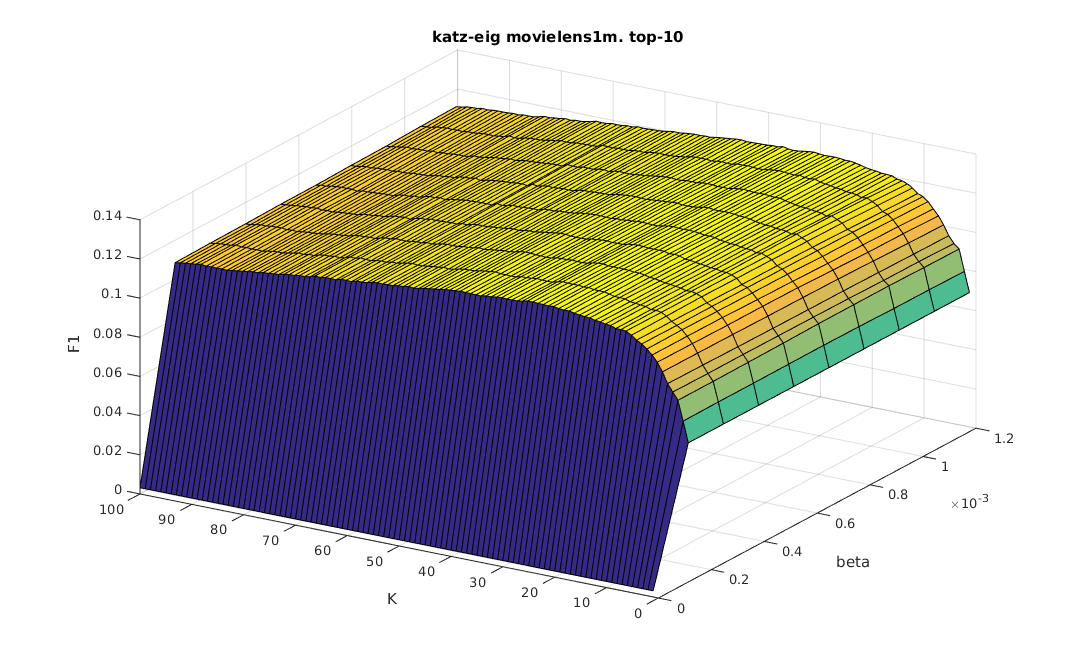
\includegraphics[width=\linewidth]{fig/katzeig_beta_k/movielens_katzeig.png}
    \captionof{figure}{\textit{movielens1m}}
\end{minipage}%
\begin{minipage}{.5\textwidth}
    \centering
    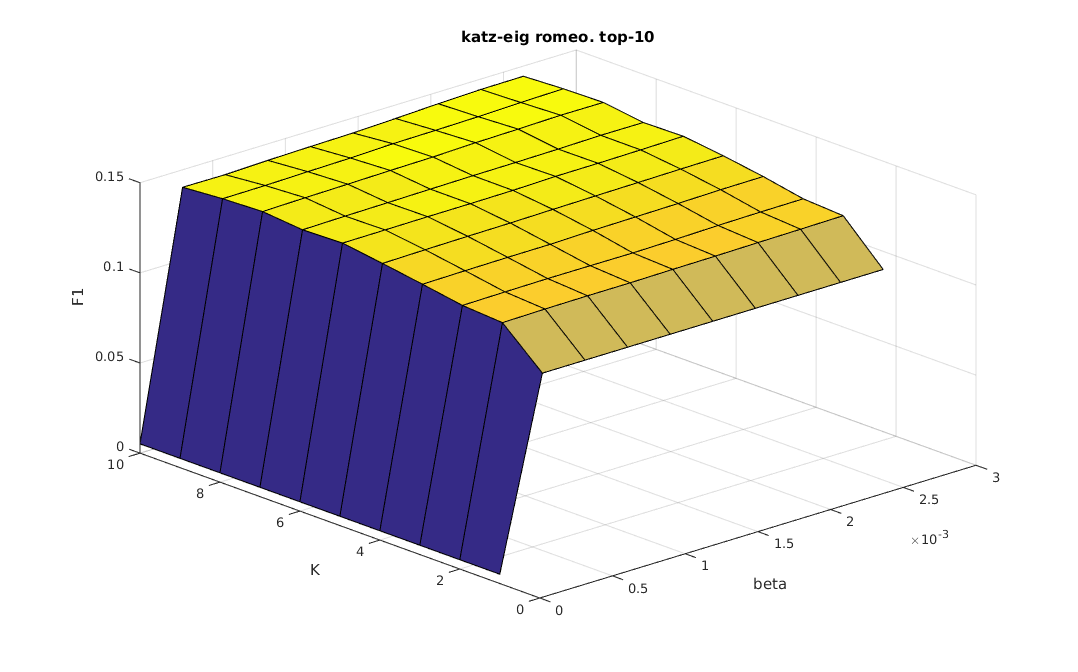
\includegraphics[width=\linewidth]{fig/katzeig_beta_k/romeo_katzeig.png}
    \captionof{figure}{\textit{romeo}}
\end{minipage}
\end{figure}




It seems like $beta$ doesn't have a very big impact on the function value. Some plots with a fixed $K$ follows to better see differences.

The range examined is $0 < \beta \leq \beta_{max} = \frac{1}{\|A_{train}\|_2}$ with a $K$ selected to fit the specific dataset. Again evaluated using \textit{Precision}, \textit{Recall} and \textit{F-measure} w.r.t. the test set using the top-10 recommendations.

\FloatBarrier

\begin{figure}[h!]
\centering
\begin{minipage}{.5\textwidth}
    \centering
    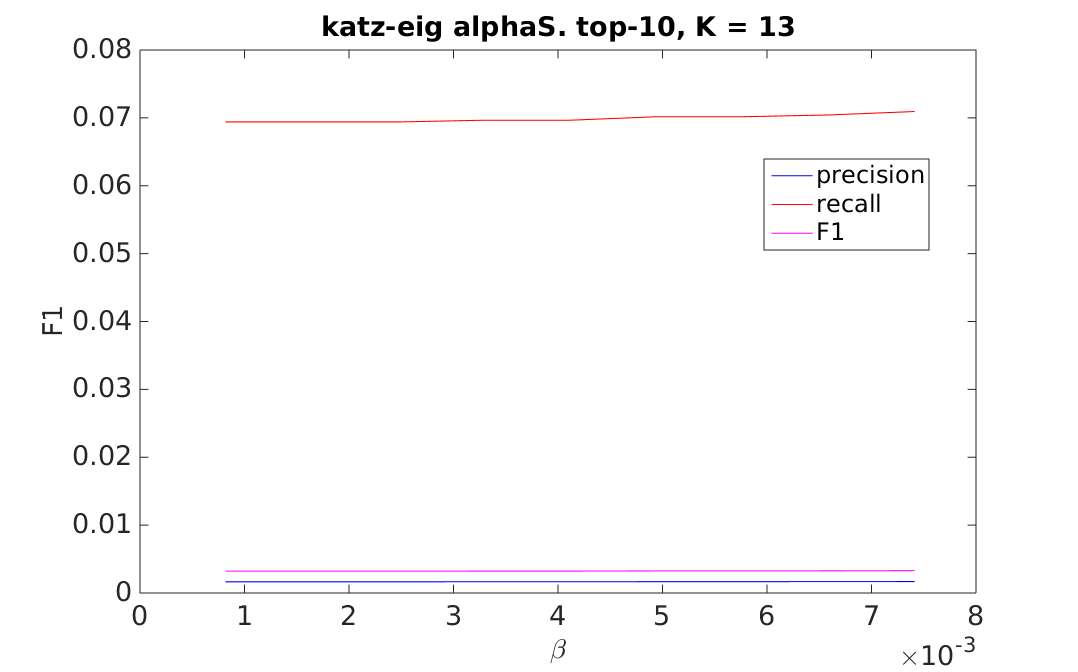
\includegraphics[width=\linewidth]{fig/katzeig_beta/alphaS_katzeig_beta.png}
    \captionof{figure}{\textit{alphaS}.
        $\beta_{max}$ is the best value with a $1.9\%$ diff between the minimum and the maximum \textit{F1} value.}
\end{minipage}%
\begin{minipage}{.5\textwidth}
    \centering
    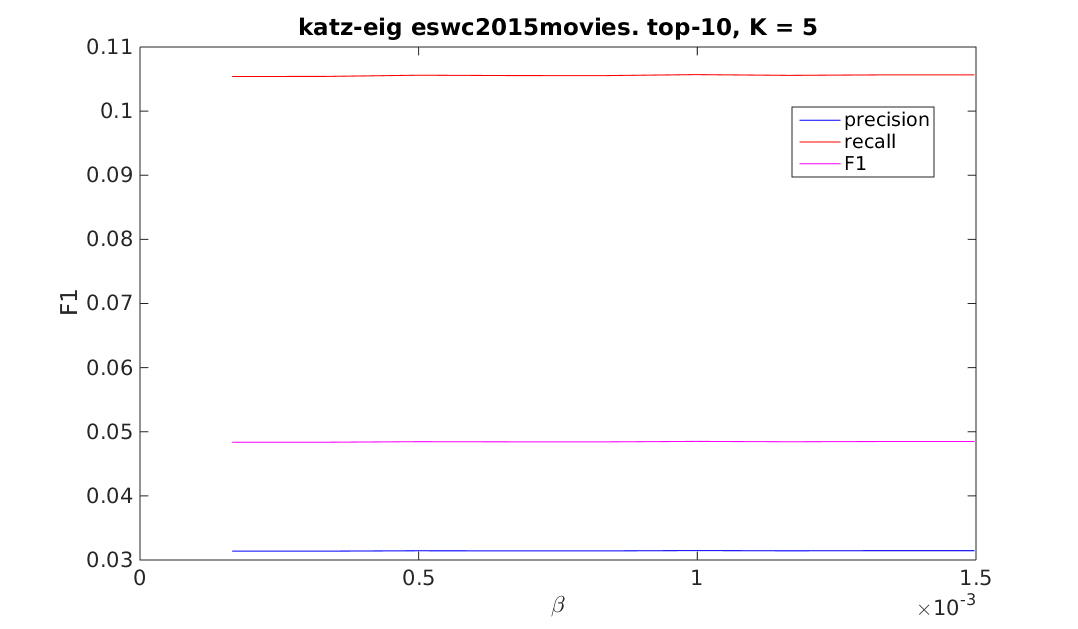
\includegraphics[width=\linewidth]{fig/katzeig_beta/eswc2015movies_katzeig_beta.png}
    \captionof{figure}{\textit{eswc2015movies}.
        $\beta_{max}$ is not the best value with a $0.3\%$ diff between the minimum and the maximum \textit{F1} value.}
\end{minipage}
\end{figure}

\begin{figure}[h!]
\centering
\begin{minipage}{.5\textwidth}
    \centering
    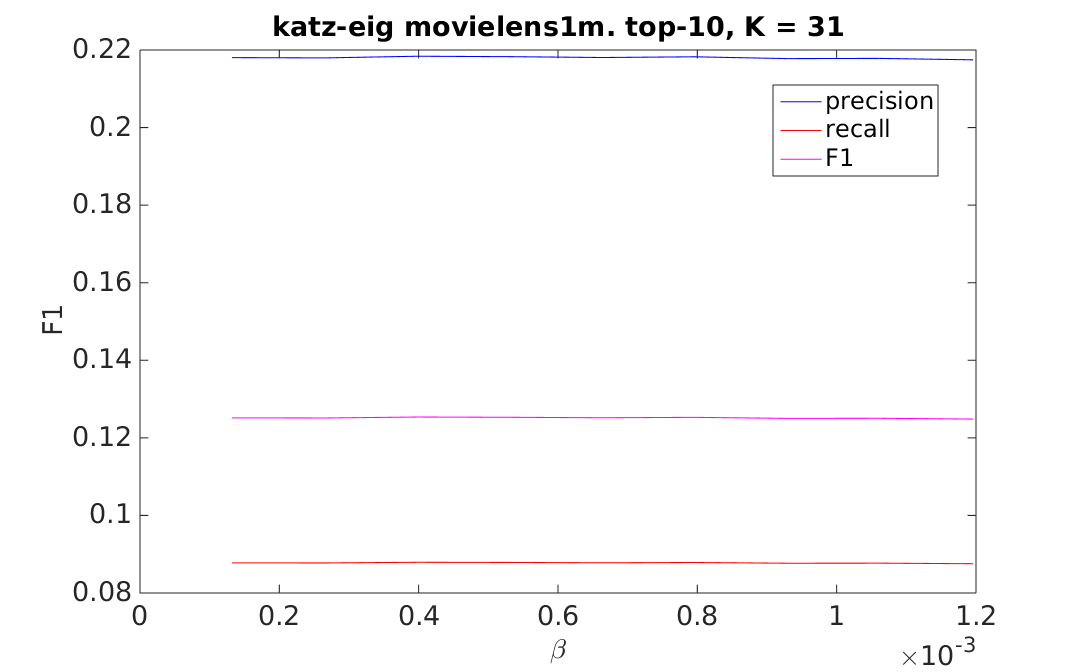
\includegraphics[width=\linewidth]{fig/katzeig_beta/movielens_katzeig_beta.png}
    \captionof{figure}{\textit{movielens1m}.
        $\beta_{max}$ is not the best value with a $0.41\%$ diff between the minimum and the maximum \textit{F1} value.}
\end{minipage}%
\begin{minipage}{.5\textwidth}
    \centering
    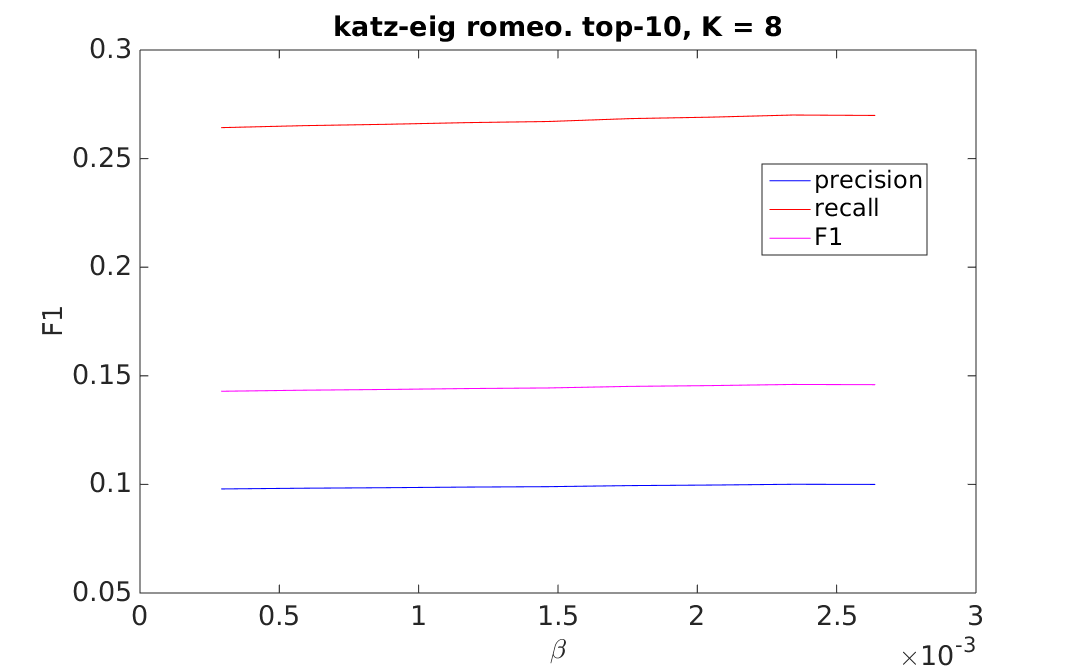
\includegraphics[width=\linewidth]{fig/katzeig_beta/romeo_katzeig_beta.png}
    \captionof{figure}{\textit{movielens1m}.
        $\beta_{max}$ is not the best value with a $2.09\%$ diff between the minimum and the maximum \textit{F1} value.}
\end{minipage}
\end{figure}

\FloatBarrier

The difference between the optimal $\beta$ and an arbitrary selected $\beta$ isn't very large. Even smaller is the difference between the optimal $\beta$ and $\beta_{max}$.  \Tableref{tab:katzeig_beta} is a summary of the evaluated values.

\begin{table}[h!]
    \centering
    \begin{tabular}{| c | r | r | r | r | l |}
        \hline
        \textbf{dataset}        & \textbf{diff between $\beta_{opt}$ and $\beta_{max}$ }    & \textbf{diff between $f_{min}$ and $f_{max}$} \\ \hline

        \textit{alphaS}         & 0~\%      & 2.0~\%    \\ \hline
        \textit{eswc2015books}  & 0~\%      & 0\%       \\ \hline
        \textit{eswc2015movies} & 0.039~\%  & 0.28~\%   \\ \hline
        \textit{movielens1m}    & 0.41~\%   & 0.41~\%   \\ \hline
        \textit{romeo}          & 0.072~\%  & 2.1~\%    \\ \hline


    \end{tabular}
    \caption{A summary of evaluating different $\beta$. $\beta_{max} = \frac{1}{\|A_{train}\|_2}$ is the maximally examined $\beta$ and $\beta_{opt}$ is the optimal $\beta$ found in the range $0 < \beta \leq \beta_{max}$. $K$ is individually optimized for the different datasets. $f_{min}$ and $f_{max}$ are the minimal and maximal \textit{F1} values obtained.}
    \label{tab:katzeig_beta}
\end{table}

\FloatBarrier

\newpage


The $K$-rank approximation represents different available models for \textit{katz-eig}. The following plots show different values of $K$, evaluated w.r.t. the test set. $\beta = \frac{1}{\|A_{train}\|}_2$ for all datasets. $K_{m}$ is the value of $K$ which gives the best \textit{F-measure} for each dataset.

\FloatBarrier

\begin{figure}[h!]
\centering
\begin{minipage}{.5\textwidth}
    \centering
    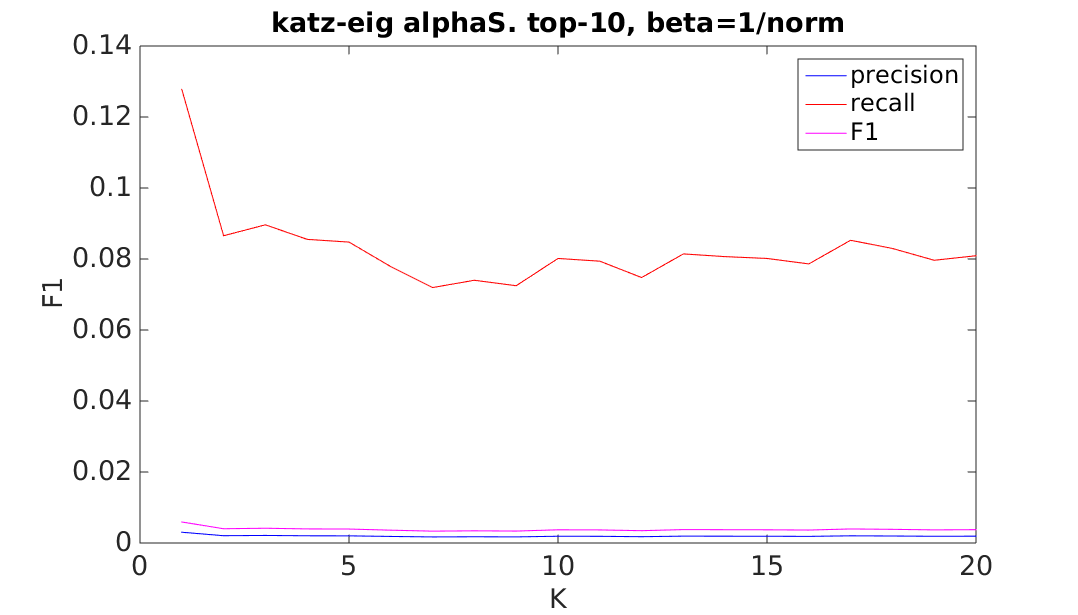
\includegraphics[width=\linewidth]{fig/katzeig_k/alphaS_katzeig_K.png}
    \captionof{figure}{\textit{alphaS} $K_{m} = 13$}
\end{minipage}%
\begin{minipage}{.5\textwidth}
    \centering
    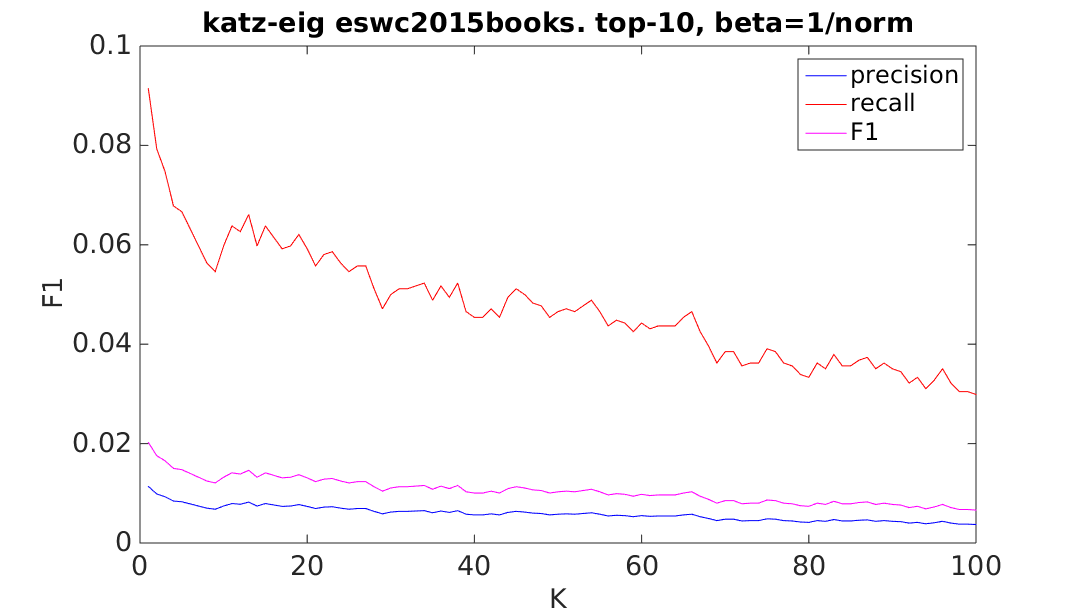
\includegraphics[width=\linewidth]{fig/katzeig_k/eswc2015books_katzeig_K.png}
    \captionof{figure}{\textit{eswc2015books} $K_{m} = 1$}
\end{minipage}
\end{figure}

\begin{figure}[h!]
\centering
\begin{minipage}{.5\textwidth}
    \centering
    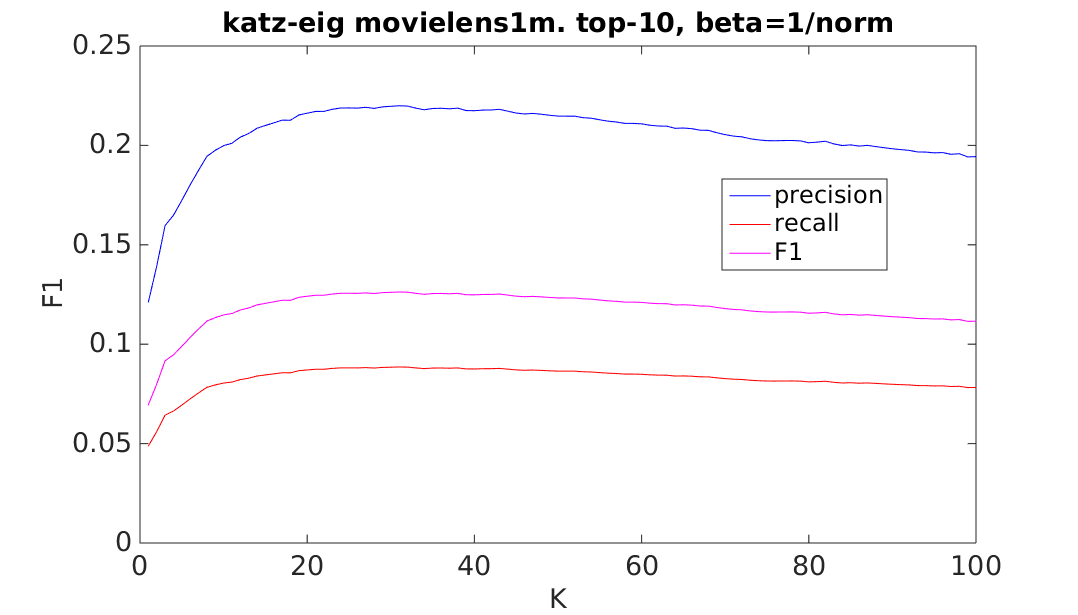
\includegraphics[width=\linewidth]{fig/katzeig_k/movielens_katzeig_K.png}
    \captionof{figure}{\textit{movielens1m} $K_{m} = 31$}
\end{minipage}%
\begin{minipage}{.5\textwidth}
    \centering
    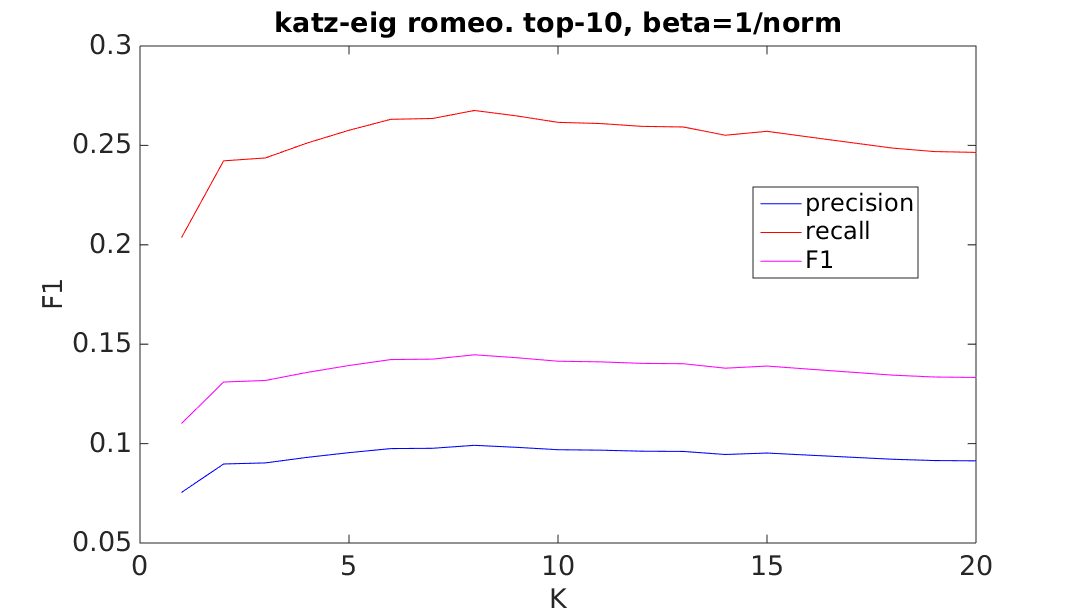
\includegraphics[width=\linewidth]{fig/katzeig_k/romeo_katzeig_K.png}
    \captionof{figure}{\textit{romeo} $K_{m} = 8$}
\end{minipage}
\end{figure}

\Warning[TODO]{ Plot of \textit{eswc2015movies}? }

%\begin{figure}[h!]
%\centering
%\begin{minipage}{.5\textwidth}
    %\centering
    %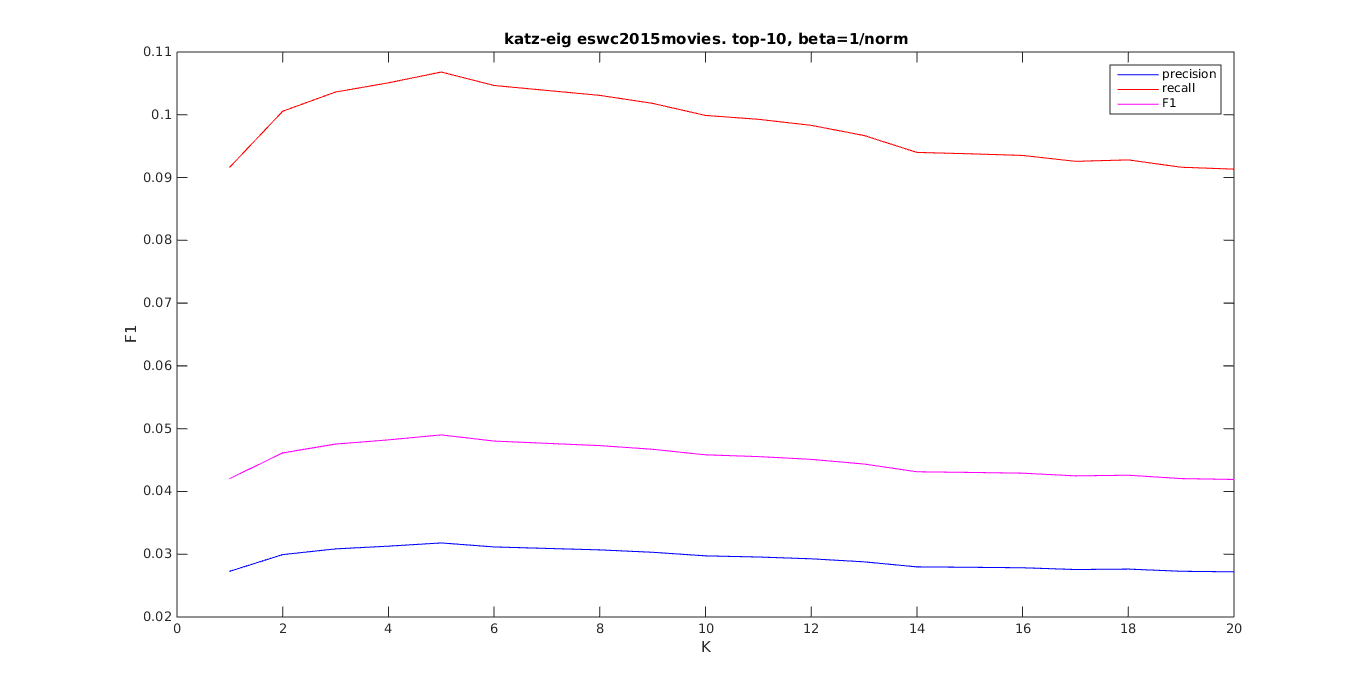
\includegraphics[width=\linewidth]{fig/katzeig_k/eswc2015movies_katzeig_K.png}
    %\captionof{figure}{\textit{eswc2015movies} $K_{m} = 5$}
%\end{minipage}%
%\begin{minipage}{.5\textwidth}
    %\centering
    %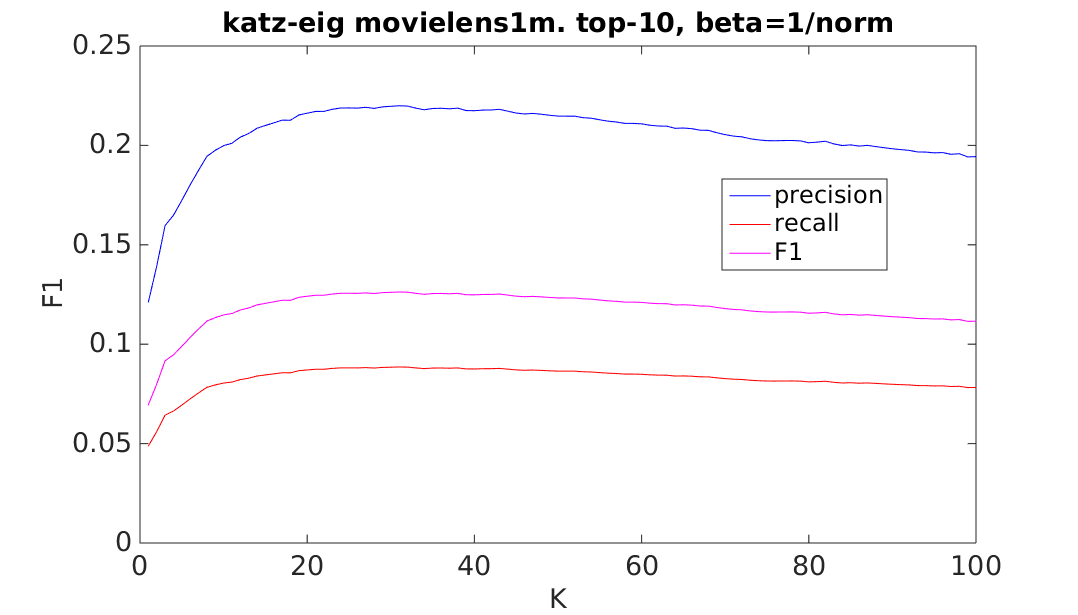
\includegraphics[width=\linewidth]{fig/katzeig_k/movielens_katzeig_K.png}
    %\captionof{figure}{\textit{movielens1m} $K_{m} = 31$}
%\end{minipage}
%\end{figure}

%\begin{figure}[h!]
%%\centering
%\begin{minipage}{.5\textwidth}
    %%\centering
    %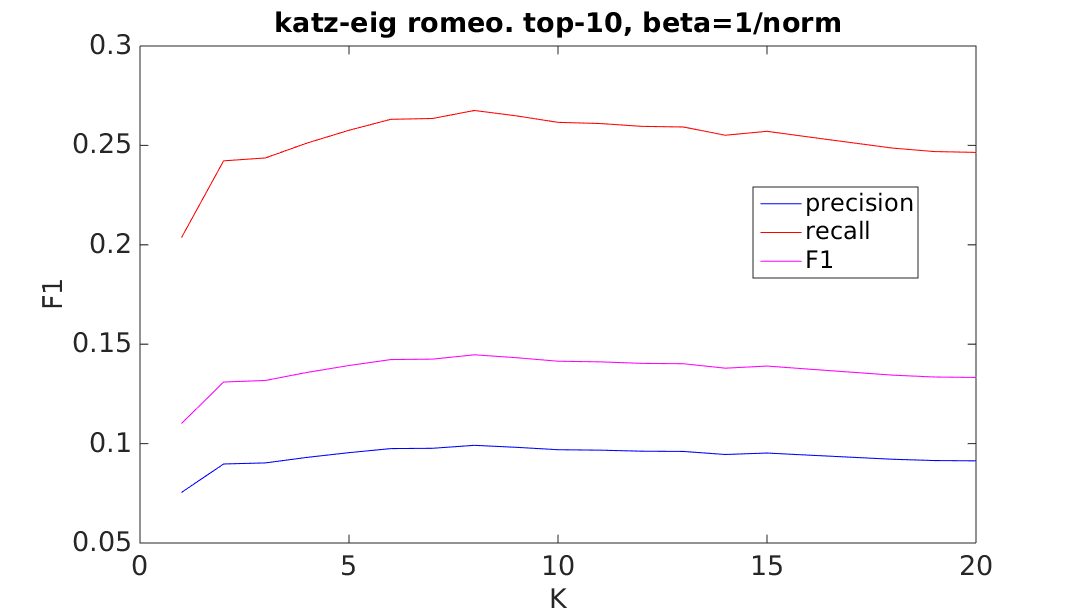
\includegraphics[width=\linewidth]{fig/katzeig_k/romeo_katzeig_K.png}
    %\captionof{figure}{\textit{romeo} $K_{m} = 8$}
%\end{minipage}%
%\end{figure}

\FloatBarrier

The function space w.r.t. $K$ is fairly smooth if not entirely convex. \textit{eswc2015books} is an outlier with a low optimal value $K = 1$ and many local optima. The other datasets display more smooth functions, but there are clear local optima with both \textit{alphaS} and \textit{romeo}.

Also of note is that the functions start to decline at different $K$. \textit{eswc2015movies} declines already at $K = 5$ but it's only at around $K = 30$ \textit{movielens1m} starts to decline. As noted earlier \textit{eswc2015books} has it's optima already at $K = 1$.




\section{Unsupervised learning}\label{sec:theory:unsuplearn}

In contrast with supervised learning, \textit{unsupervised learning} doesn't have an expected output to learn from. Instead the task is to learn patterns in the input without any feedback.

The most common unsupervised learning task is \textit{clustering}: detecting potentially useful clusters, or groups, of input examples. \citep{norvigAI}



